\section{Motion Representation and Conditioning}
\label{sec:preliminaries}
\subsection{Kimodo representation}
Kimodo~\cite{kimodo} is a controllable diffusion-based motion generator with pretrained human and G1 skeleton models. Its root denoiser predicts global root motion, then its body denoiser generates articulated motion conditioned on the root's local representation. We use the G1 model pretrained on human motion retargeted with the SOMA retargeter~\cite{saito2026somaunifyingparametrichuman}.

For $J$ joints, each frame is represented by
\begin{equation}
\mathbf{x}_n=[\mathbf{r}^p_n,\mathbf{r}^a_n,\mathbf{j}^p_n,\mathbf{j}^v_n,\mathbf{j}^a_n,\mathbf{f}_n]
\in\mathbb{R}^{12J+9}.
\end{equation}
The root's initial horizontal position is centered at the origin. Root position $\mathbf{r}^p_n\in\mathbb{R}^3$ smooths the horizontal pelvis coordinates while preserving vertical height; heading is $\mathbf{r}^a_n=[\cos\psi_n,\sin\psi_n]$. Joint positions use horizontal offsets from the smoothed root and absolute vertical coordinates, with world-aligned axes. Joint velocities are derived from global positions. Each global joint orientation uses a continuous six-dimensional representation. Four binary contact values describe the left/right heel and toe. Root features are $[\mathbf{r}^p_n,\mathbf{r}^a_n]$; the remaining groups form the body representation. Feature-wise observation masks allow only available history values to be imposed as constraints.

\subsection{ControlNet adaptation}
ControlNet~\cite{zhang2023adding} freezes a pretrained denoiser and injects features from a trainable branch through zero-initialized projections. For frozen layer $F_l$, control layer $G_{\phi,l}$, and conditioning $\mathbf{c}$,
\begin{align}
\mathbf{h}^{\rm ctrl}_{l+1}&=G_{\phi,l}(\mathbf{h}^{\rm ctrl}_l,\mathbf{c}),\\
\mathbf{h}^{\rm lock}_{l+1}&=F_l(\mathbf{h}^{\rm lock}_l)+\mathcal{Z}_l(\mathbf{h}^{\rm ctrl}_{l+1}).
\end{align}
The residual is initially zero. In Kimodo-Policy, control branches adapt Transformer root/body denoisers, rather than an image U-Net. Cross-attention retrieves image content using future-motion queries, while a token-axis MLP maps visual tokens to the future horizon. The resulting hints enter future tokens only. History is restored before each denoising step; padding and unavailable features are masked. This history constraint and the zero-initialized visual residual serve different purposes: temporal anchoring and conservative initialization, respectively.

\section{Data and Training Details}
\subsection{Policy-pretraining corpus}
Our 419-hour corpus combines HIW-500, 14 UniFoLM-WBT G1 subsets, and Humanoid Everyday~\cite{humanoid_everyday}. This is robot \emph{policy} pretraining, separate from the prior motion-generator training. HIW-500 contains teleoperated demonstrations in real homes. The UniFoLM-WBT snapshot includes the BrainCo subsets \emph{Collect Plates into Dishwasher}, \emph{Make the Bed}, \emph{Pick Up Medicine}, and \emph{Pickup Pillow}; the Dex1 subset \emph{Put Clothes into Washing Machine}; and the Inspire subsets \emph{Clean the Living Room}, \emph{Collect Clothes (MainCamOnly)}, \emph{Pick Up Drinks}, \emph{Pickup Pillow (MainCamOnly)}, \emph{Put Clothes into Basket}, \emph{Put Clothes into Washing Machine}, \emph{Put Clothes into Washing Machine (MainCamOnly)}, \emph{Put Drinks into Fridge}, and \emph{Put Vegetables into Basket}. Entries released after corpus construction are excluded. Humanoid Everyday supplies 10.3K trajectories, over three million frames, and 260 tasks. Figure~\ref{fig:corpus} visualizes the source composition.

Each training example includes an egocentric image, a language instruction, 100 motion-history frames, and a 50-frame target at 30\,Hz. Bilateral open/closed hand states provide a common two-dimensional supervision space across source hand morphologies. Trajectories are converted to Kimodo's kinematic representation.

\begin{figure*}[t]\centering
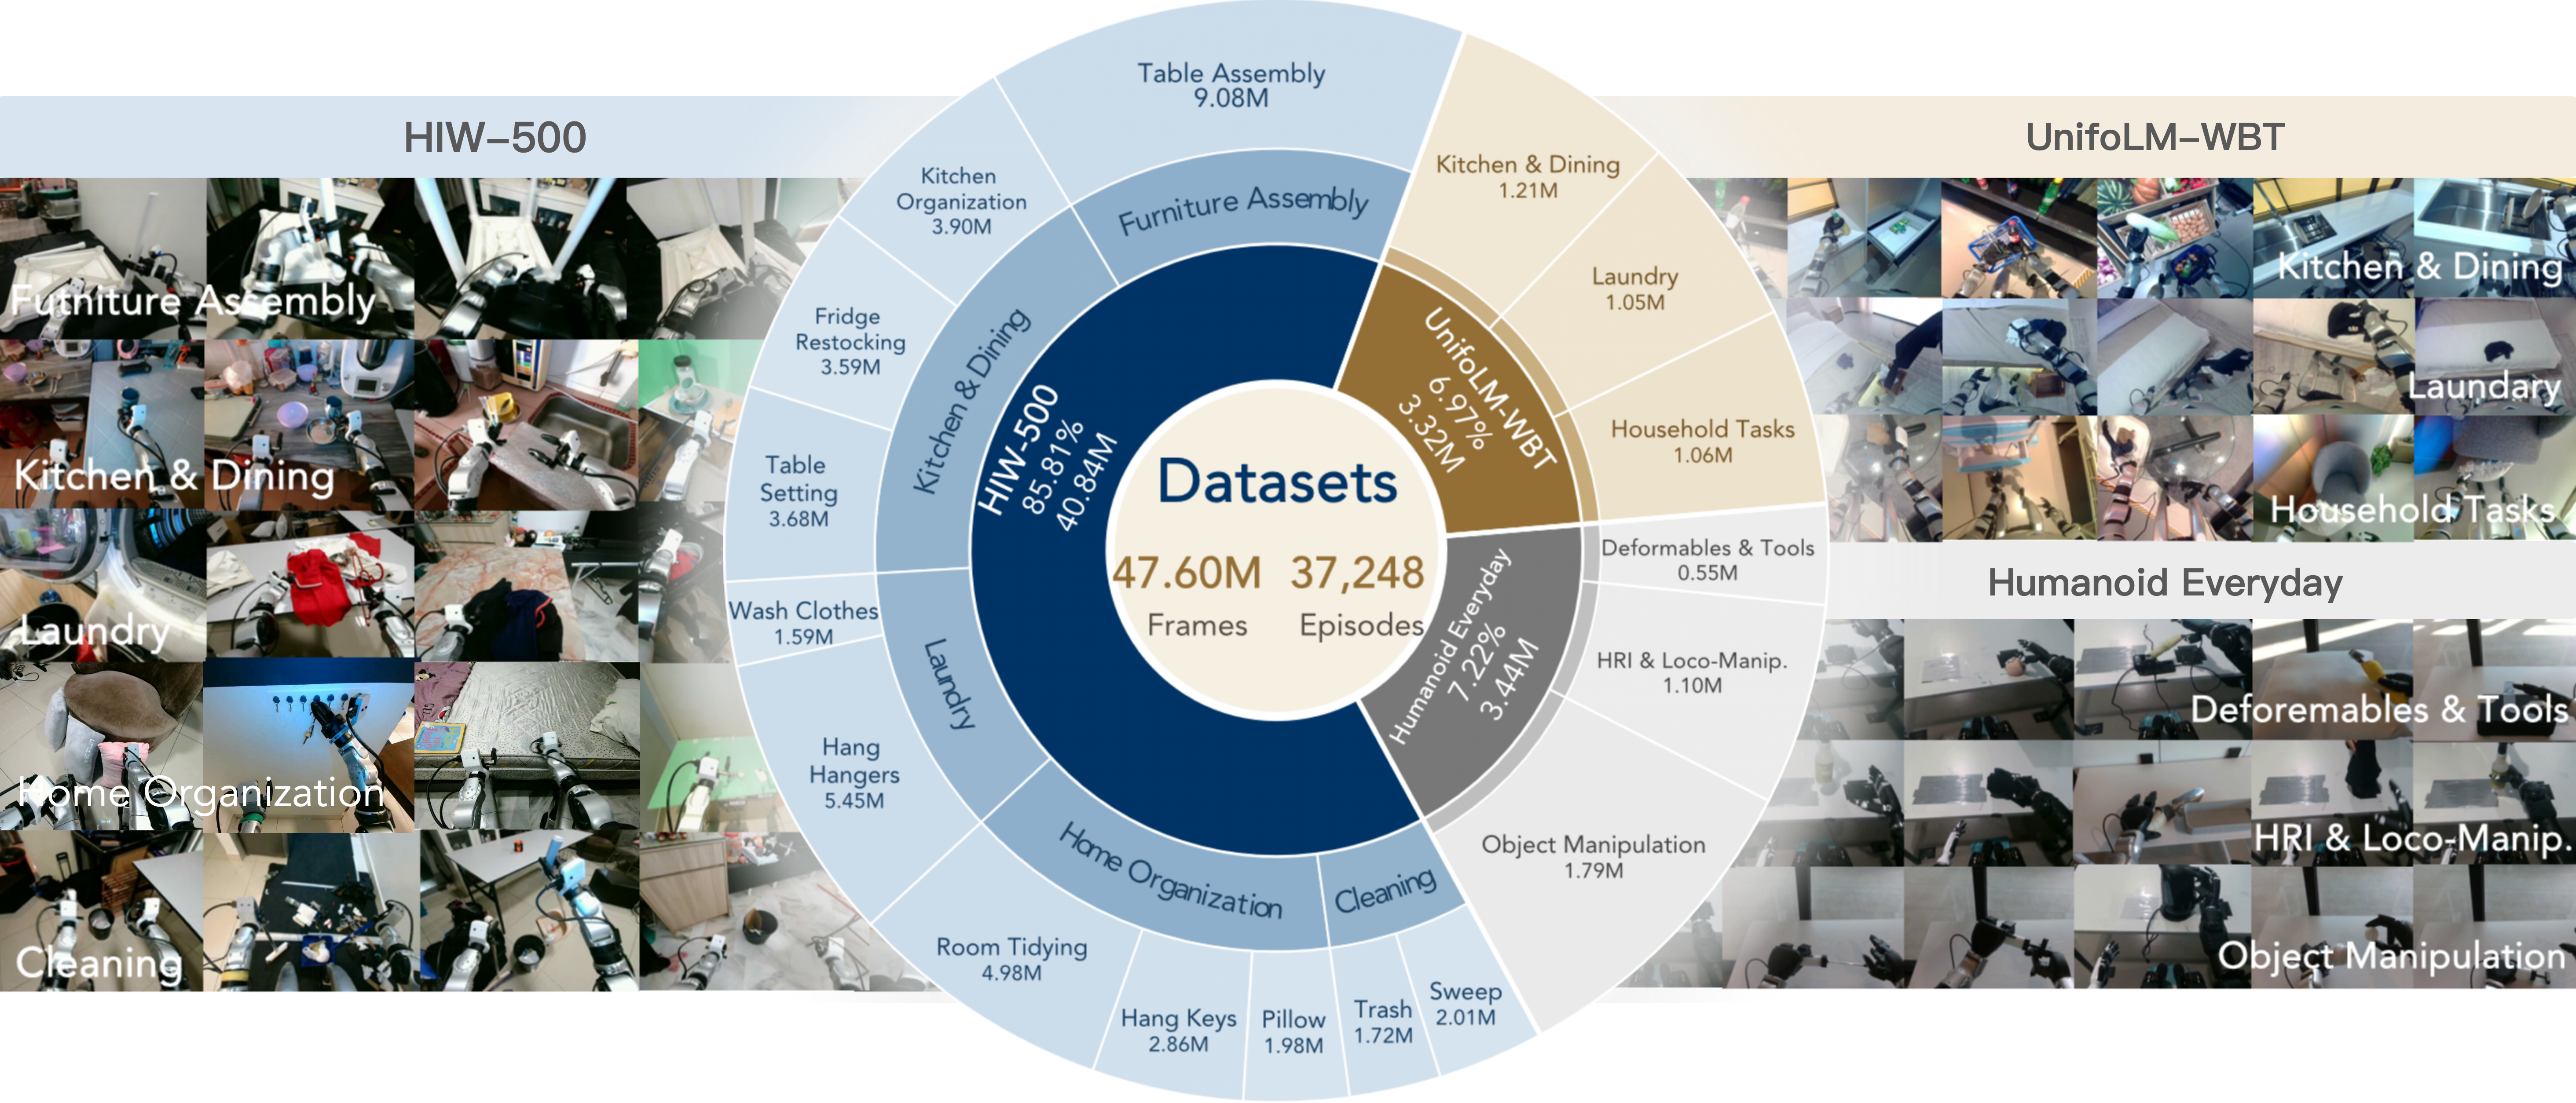
\includegraphics[width=\textwidth]{image/pretrain.png}
\caption{\textbf{Policy-pretraining corpus.} Source visualization of HIW-500, the selected UniFoLM-WBT snapshot, and Humanoid Everyday. Dataset composition refers to the corpus construction snapshot.}
\label{fig:corpus}\end{figure*}

\subsection{Optimization}
Policy pretraining runs for 1,000k steps on 16 NVIDIA H200 GPUs, approximately 60 hours, with bfloat16 precision and global batch size 1024. AdamW uses weight decay 0.01, a $3\times10^{-5}$ learning rate for ControlNet Transformer layers, and $10^{-4}$ for conditioning modules and HandNet. A cosine schedule uses 1\% warm-up and a minimum learning rate of 10\% of the initial value.

Target-task fine-tuning uses four GPUs and bfloat16 precision. HumanoidArena single-task models use batch size 64 for 200k steps; the joint model uses batch size 128 for 500k steps. SIMPLE uses batch size 64 for 200k steps, and physical-robot policies use batch size 32 for 50k steps. Both initialization variants use the same pretrained motion backbone and target-task schedule. The four-layer ControlNet detaches root-control inputs to the body branch.

The three learning rates (ControlNet Transformer layers, conditioning modules, HandNet) are $(3\times10^{-5},10^{-4},10^{-4})$ for HumanoidArena and $(10^{-5},3\times10^{-5},3\times10^{-5})$ for SIMPLE and the physical robot. Weight decay, warm-up, and cosine minimum follow pretraining. Root/body/hand reconstruction uses MSE with weights 4/1/1, and the hand-transition $\ell_1$ term has weight 0.2. Motion losses mask padding; hand losses also mask absent labels. Transition loss requires both neighboring labels, including the observed-to-future boundary. For continuous control, closure residuals are converted back to closure values before the transition loss.

SIMPLE uses color jitter and continuous hand targets. Physical-robot training uses color jitter and random crops, with binary commands conditioned on measured hand closure. Neither target-task regime updates Kimodo or DINOv3.

\section{Evaluation and Deployment}
\subsection{Benchmark tasks}
HumanoidArena~\cite{humanoidarena,sonic} supplies 700 successful demonstrations, 100 for each of seven tasks (Fig.~\ref{fig:arena}). They contain synchronized egocentric RGB, proprioceptive states, and whole-body targets. The HOI group contains Football, DoubleDesk, and P\&Pbox; the HSI group contains OpenDoor, SitSofa, Boxing, and VisNavi. We report both independent and joint training.

The source SIMPLE snapshot contains 18 released tasks out of 60 described in its paper~\cite{simple}. Our eight-task subset is shown in Fig.~\ref{fig:simple}. L0--L2 introduce progressively stronger visual, lighting, and target-pose variation. We report ten trials at each level, preserving all trial counts in Tables~\ref{tab:simple_a} and~\ref{tab:simple_b}. Missing literature results remain unreported rather than receiving zero scores.

\begin{figure*}[t]\centering
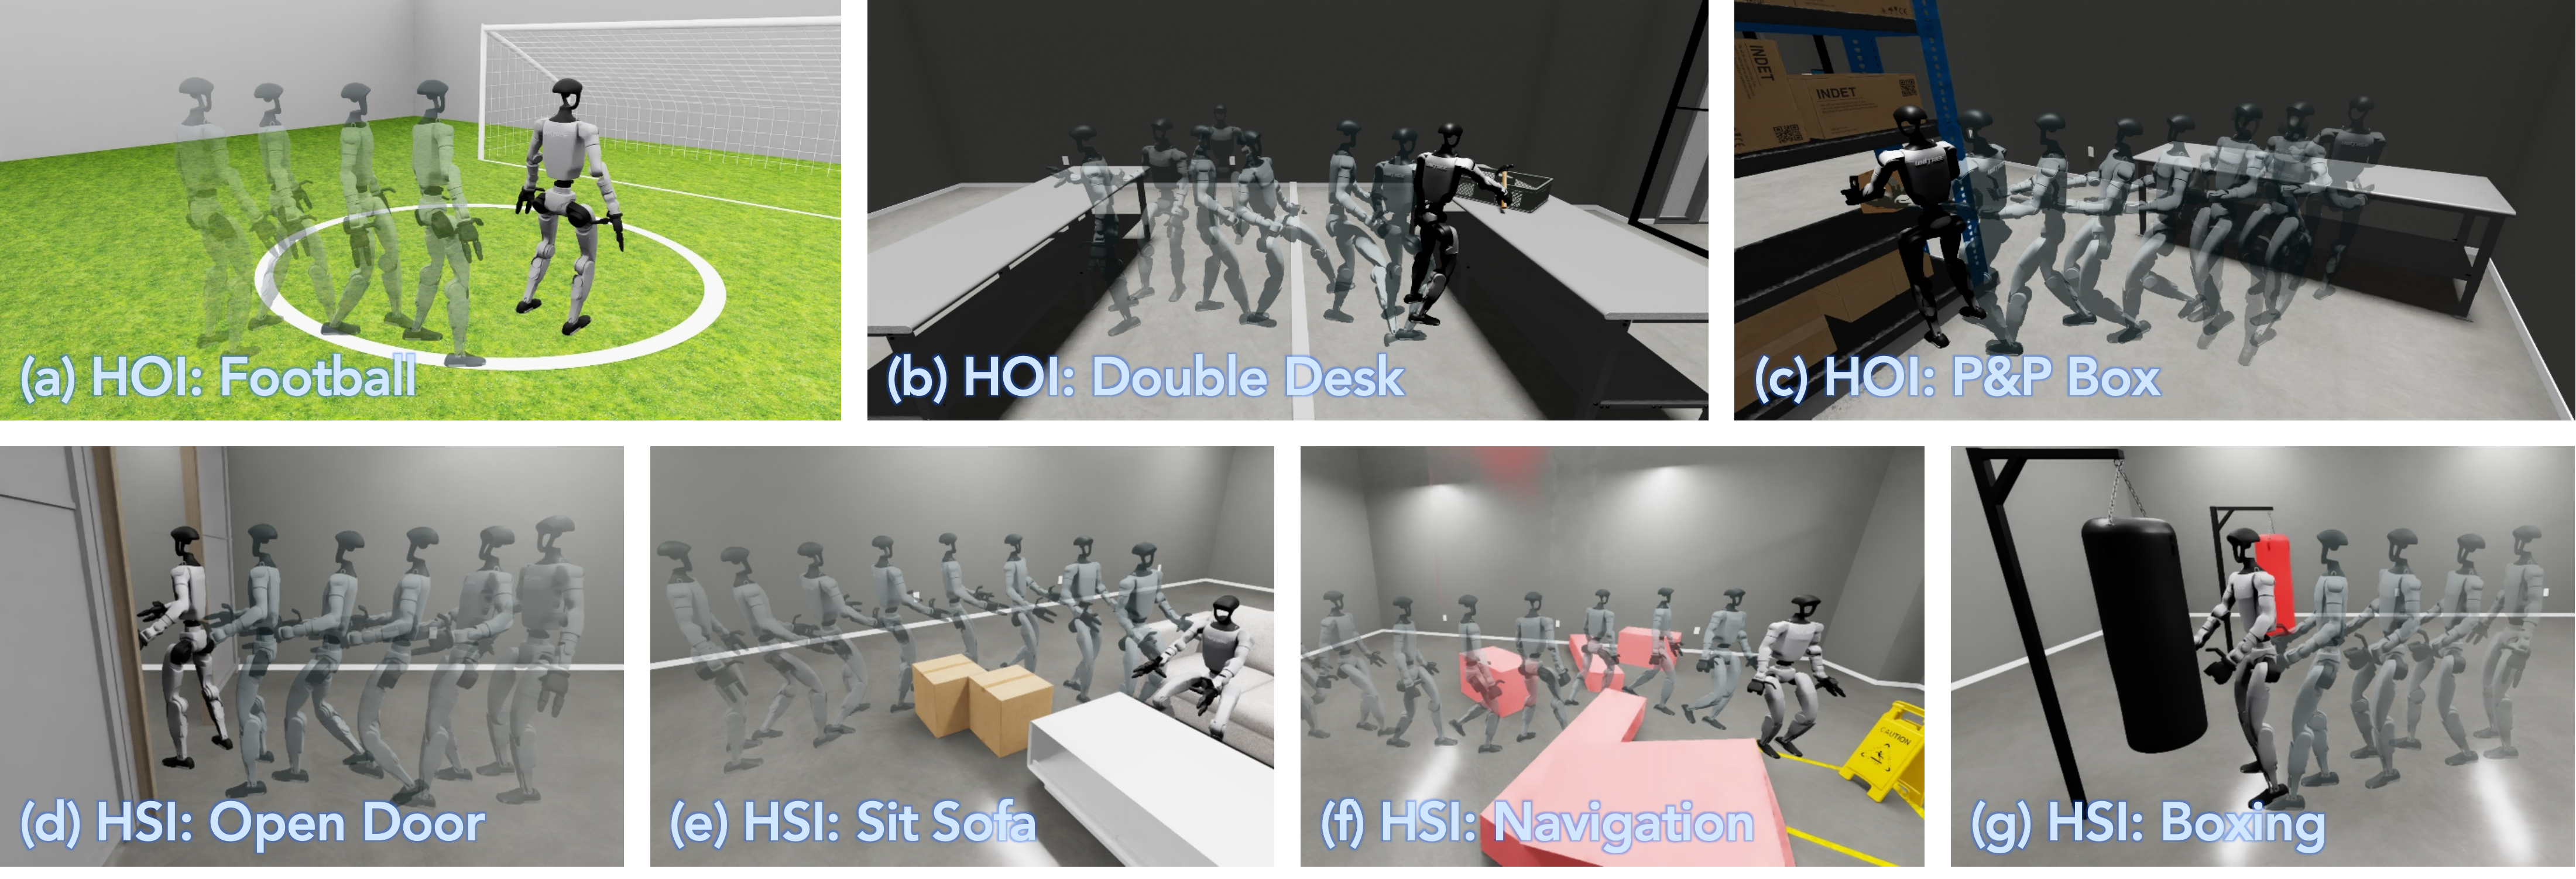
\includegraphics[width=\textwidth]{image/arena.png}
\caption{\textbf{HumanoidArena tasks.} Object and scene interactions require locomotion, posture changes, and manipulation.}
\label{fig:arena}\end{figure*}
\begin{figure*}[t]\centering
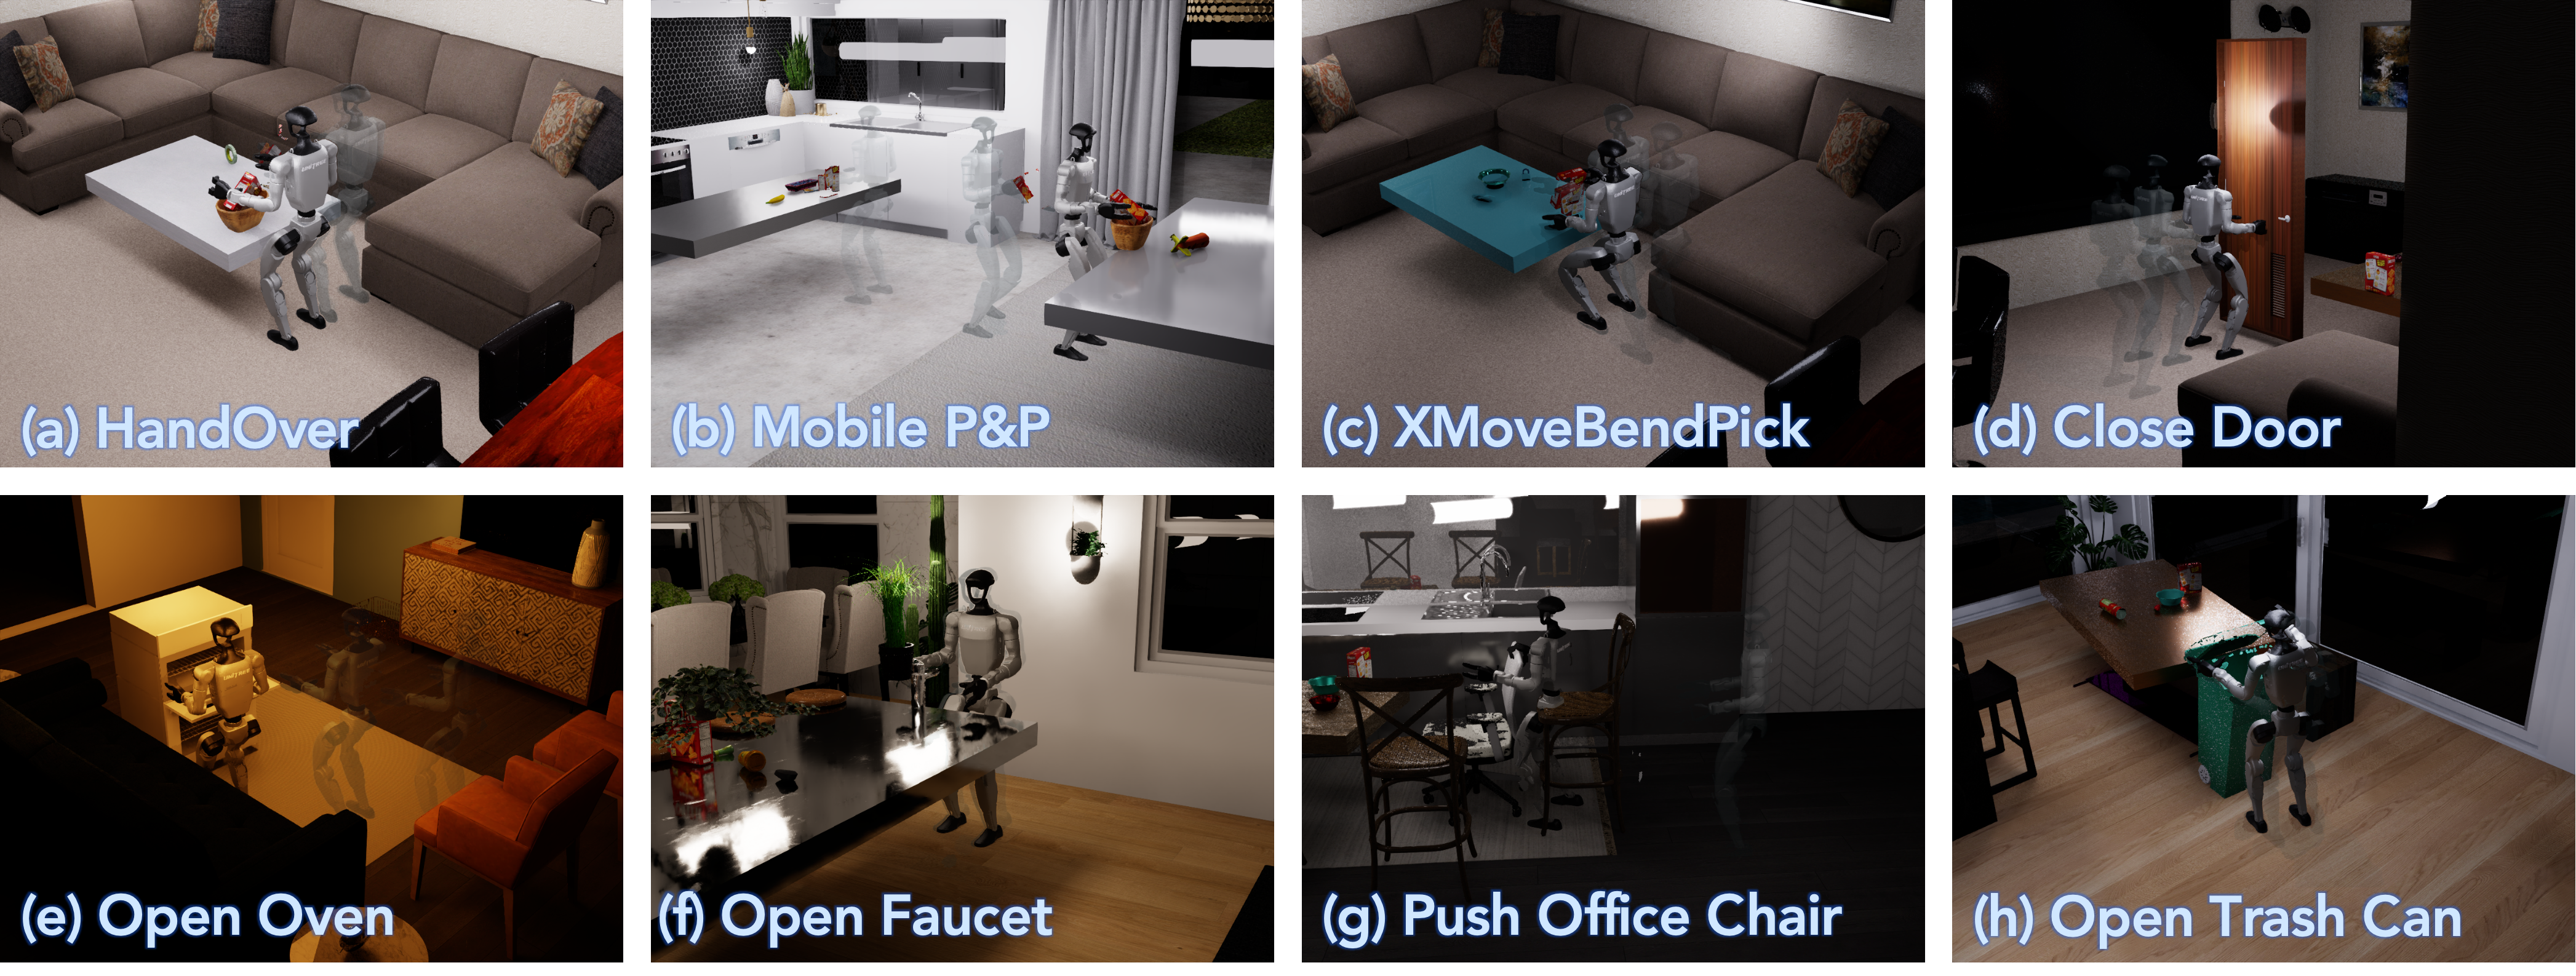
\includegraphics[width=\textwidth]{image/simple.png}
\caption{\textbf{SIMPLE task subset.} Handover, Mobile P\&P, XMoveBendPick, CloseDoor, OpenOven, OpenFaucet, Push Office Chair, and OpenTrashCan.}
\label{fig:simple}\end{figure*}

\subsection{Physical data collection and execution}
The teleoperation system extends NVIDIA Isaac-GR00T's data-preparation pipeline~\cite{grootn1}. Operators use a PICO 4 Ultra headset, hand controllers, and body trackers for whole-body and lower-limb tracking. The humanoid carries an Intel RealSense D435i and Dex3-1 hands. We collect 25--30 demonstrations for each of eight tasks and store them in LeRobot v2.1-compatible form~\cite{cadene2026lerobotopensourcelibraryendtoend}, with additional motion and control fields. Hardware and chunk execution are depicted in Fig.~\ref{fig:deployment}.

At inference, one RTX 4090 performs ten DDIM steps to predict 50 frames at 30\,Hz. Fifteen frames (0.5\,s) are executed per update on HumanoidArena and the robot. SIMPLE uses either 15 or 50 frames depending on the setting. The SONIC tracker runs at 50\,Hz, and real-time chunking~\cite{rtc} is enabled only on the physical robot. The diagram's inference timing illustrates the deployment pipeline rather than a separately controlled latency benchmark. The source does not isolate RTC's effect from the other physical-deployment components.

\begin{figure*}[t]\centering
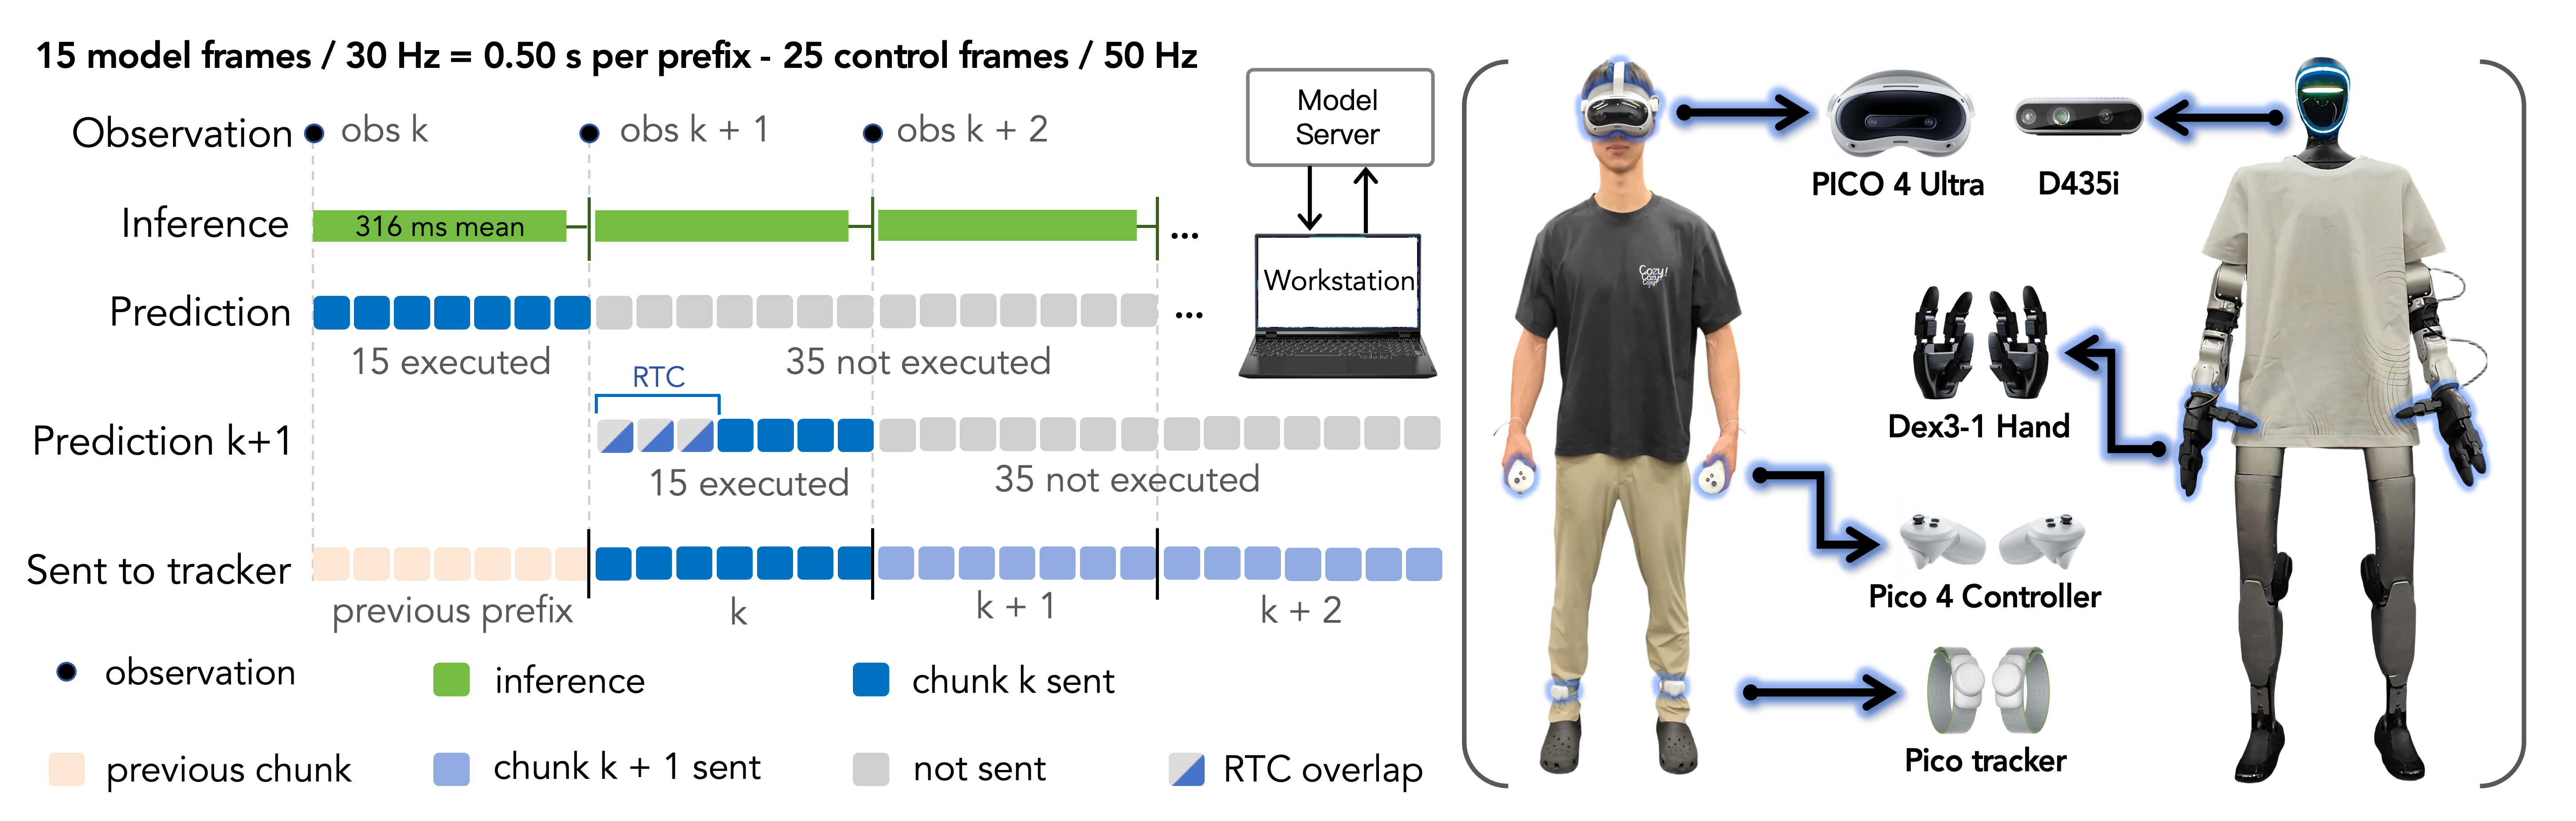
\includegraphics[width=\textwidth]{image/post-train.png}
\caption{\textbf{Deployment timing and hardware.} Left: a 15-frame execution prefix, asynchronous prediction, and RTC overlap between chunks. Right: the model server, workstation, PICO teleoperation equipment, D435i camera, and Dex3-1 hands.}
\label{fig:deployment}\end{figure*}

\section{Complete Benchmark Results}
Tables~\ref{tab:supp_single_hoi}--\ref{tab:supp_multi_hsi} reproduce all source HumanoidArena entries, split into object- and scene-interaction columns for readability. Means and deviations are retained as reported; minor differences between displayed task means and aggregates can arise from rounding. The multi-task comparison includes literature results from HuGe~\cite{liu2026huge} and Language-Forcing~\cite{li2026languageforcing}; these are not re-runs under an identical training budget. AFR is absent for these literature rows. Baseline methods include ACT~\cite{ACT}, DP~\cite{chi2023diffusionpolicy}, flow matching~\cite{FM_objective}, $\pi_{0.5}$~\cite{pi05}, Fast-WAM~\cite{yuan2026fastwam}, LingBot-VA~\cite{li2026lingbotva}, GR00T~\cite{grootn1}, and GigaWorld-Policy~\cite{gigaworld2026policy05}.

\begin{table*}[t]
\centering\small
\caption{\textbf{Single-task HumanoidArena: HOI.} All values are percentages; deviations are reproduced where available. For our rows, $^{*}$ means additional policy pretraining. Deviations are retained as reported; the source does not specify their aggregation procedure.}
\label{tab:supp_single_hoi}
\setlength{\tabcolsep}{4pt}
\begin{tabular}{lrrrrr}\toprule
Method & AFR & Football & DoubleDesk & P\&Pbox & HOI mean\\\midrule
ACT & 8.57\% & 16.7$\pm$6.2\% & 18.3$\pm$4.7\% & 56.7$\pm$6.2\% & 30.56$\pm$19.36\%\\
DP & 8.33\% & 45.0$\pm$10.8\% & 36.7$\pm$4.7\% & 75.0$\pm$4.1\% & 52.22$\pm$17.97\%\\
FM & 5.71\% & 13.3$\pm$2.4\% & 38.3$\pm$4.7\% & 73.3$\pm$6.2\% & 41.67$\pm$25.06\%\\
$\pi_{0.5}$ & 5.24\% & 10.0$\pm$4.1\% & 43.3$\pm$6.2\% & 71.7$\pm$11.8\% & 41.67$\pm$26.46\%\\
Ours & 4.29\% & 28.3$\pm$6.2\% & 40.0$\pm$0.0\% & 80.0$\pm$4.1\% & 49.44$\pm$22.54\%\\
Ours$^{*}$ & 4.29\% & 26.7$\pm$4.7\% & 28.3$\pm$2.4\% & 78.3$\pm$8.5\% & 44.44$\pm$24.66\%\\
\bottomrule\end{tabular}\end{table*}

\begin{table*}[t]
\centering\small
\caption{\textbf{Single-task HumanoidArena: HSI.} All values are percentages; deviations are reproduced where available. For our rows, $^{*}$ means additional policy pretraining. Deviations are retained as reported; the source does not specify their aggregation procedure.}
\label{tab:supp_single_hsi}
\setlength{\tabcolsep}{4pt}
\begin{tabular}{lrrrrrr}\toprule
Method & OpenDoor & SitSofa & Boxing & VisNavi & HSI mean & Overall\\\midrule
ACT & 78.3$\pm$9.4\% & 73.3$\pm$8.5\% & 56.7$\pm$6.2\% & 33.3$\pm$2.4\% & 60.42$\pm$18.98\% & 47.61\%\\
DP & 85.0$\pm$10.8\% & 78.3$\pm$14.3\% & 76.7$\pm$2.4\% & 23.3$\pm$6.2\% & 65.83$\pm$26.52\% & 60\%\\
FM & 70.0$\pm$4.1\% & 15.0$\pm$14.7\% & 70.0$\pm$8.2\% & 38.3$\pm$14.3\% & 48.33$\pm$26.94\% & 45.46\%\\
$\pi_{0.5}$ & 66.7$\pm$6.2\% & 73.3$\pm$2.4\% & 70.0$\pm$0.0\% & 23.3$\pm$6.2\% & 58.33$\pm$20.85\% & 51.19\%\\
Ours & 90.0$\pm$4.1\% & 100.0$\pm$0.0\% & 73.3$\pm$13.1\% & 75.0$\pm$10.8\% & 84.58$\pm$14.06\% & 69.51\%\\
Ours$^{*}$ & 93.3$\pm$2.4\% & 96.7$\pm$2.4\% & 70.0$\pm$8.2\% & 76.7$\pm$18.9\% & 84.17$\pm$15.25\% & 67.14\%\\
\bottomrule\end{tabular}\end{table*}

\begin{table*}[t]
\centering\small
\caption{\textbf{Multi-task HumanoidArena: HOI.} All values are percentages; deviations are reproduced where available. HuGe rows come from~\cite{liu2026huge}; $\dagger$ rows from~\cite{li2026languageforcing}. For our rows, $^{*}$ means additional policy pretraining. Deviations are retained as reported; the source does not specify their aggregation procedure.}
\label{tab:supp_multi_hoi}
\setlength{\tabcolsep}{4pt}
\begin{tabular}{lrrrrr}\toprule
Method & AFR & Football & DoubleDesk & P\&Pbox & HOI mean\\\midrule
ACT & 7.4\% & 20.0$\pm$4.1\% & 30.0$\pm$4.1\% & 60.0$\pm$12.2\% & 36.7$\pm$18.7\%\\
DP & 7.1\% & 53.3$\pm$6.2\% & 35.0$\pm$10.8\% & 0.0$\pm$0.0\% & 29.4$\pm$23.3\%\\
FM & 7.1\% & 21.7$\pm$8.5\% & 20.0$\pm$7.1\% & 0.0$\pm$0.0\% & 13.9$\pm$11.7\%\\
$\pi_{0.5}$ & 6.4\% & 10.0$\pm$7.1\% & 30.0$\pm$7.1\% & 75.0$\pm$4.1\% & 38.3$\pm$27.9\%\\
HuGe-OFT$^{*}$ & --- & 48.33\% & 0.00\% & 53.33\% & 33.89\%\\
HuGe-GR00T$^{*}$ & --- & 71.67\% & 15.00\% & 81.67\% & 56.11\%\\
HuGe-Pi$^{*}$ & --- & 63.33\% & 11.67\% & 76.67\% & 50.56\%\\
Fast-WAM$^{\dagger}$ & --- & 46.25\% & 45.00\% & 73.75\% & 55.00\%\\
LingBot-VA$^{\dagger}$ & --- & 51.67\% & 41.25\% & 77.92\% & 56.95\%\\
GR00T N1.7$^{\dagger}$ & --- & 63.75\% & 49.58\% & 73.33\% & 62.22\%\\
GigaWorld-Policy$^{\dagger}$ & --- & 62.08\% & 52.50\% & 65.83\% & 60.14\%\\
Ours & 5.0\% & 35.0$\pm$7.1\% & 40.0$\pm$0.0\% & 80.0$\pm$4.1\% & 51.7$\pm$20.7\%\\
Ours$^{*}$ & 4.3\% & 40.0$\pm$4.1\% & 38.3$\pm$2.4\% & 90.0$\pm$4.1\% & 56.1$\pm$24.2\%\\
\bottomrule\end{tabular}\end{table*}

\begin{table*}[t]
\centering\small
\caption{\textbf{Multi-task HumanoidArena: HSI.} All values are percentages; deviations are reproduced where available. HuGe rows come from~\cite{liu2026huge}; $\dagger$ rows from~\cite{li2026languageforcing}. For our rows, $^{*}$ means additional policy pretraining. Deviations are retained as reported; the source does not specify their aggregation procedure.}
\label{tab:supp_multi_hsi}
\setlength{\tabcolsep}{4pt}
\begin{tabular}{lrrrrrr}\toprule
Method & OpenDoor & SitSofa & Boxing & VisNavi & HSI mean & Overall\\\midrule
ACT & 58.3$\pm$2.4\% & 21.7$\pm$2.4\% & 58.3$\pm$10.3\% & 28.3$\pm$4.7\% & 41.7$\pm$17.8\% & 39.5\%\\
DP & 83.3$\pm$6.2\% & 83.3$\pm$4.7\% & 21.7$\pm$30.6\% & 50.0$\pm$14.7\% & 59.6$\pm$31.1\% & 46.7\%\\
FM & 76.7$\pm$2.4\% & 48.3$\pm$6.2\% & 18.3$\pm$25.9\% & 38.3$\pm$6.2\% & 45.4$\pm$25.1\% & 31.9\%\\
$\pi_{0.5}$ & 85.0$\pm$4.1\% & 70.0$\pm$14.7\% & 71.7$\pm$12.5\% & 35.0$\pm$4.1\% & 65.4$\pm$21.1\% & 53.8\%\\
HuGe-OFT$^{*}$ & 75.00\% & 55.00\% & 73.33\% & 73.33\% & 69.17\% & 54.05\%\\
HuGe-GR00T$^{*}$ & 95.00\% & 78.33\% & 68.33\% & 56.67\% & 74.58\% & 66.67\%\\
HuGe-Pi$^{*}$ & 88.33\% & 83.33\% & 68.33\% & 63.33\% & 75.83\% & 65.00\%\\
Fast-WAM$^{\dagger}$ & 85.42\% & 74.58\% & 67.92\% & 35.00\% & 65.73\% & 61.13\%\\
LingBot-VA$^{\dagger}$ & 84.58\% & 77.08\% & 72.92\% & 52.08\% & 71.67\% & 65.36\%\\
GR00T N1.7$^{\dagger}$ & 82.08\% & 76.67\% & 76.67\% & 65.83\% & 75.31\% & 69.70\%\\
GigaWorld-Policy$^{\dagger}$ & 90.83\% & 74.17\% & 73.33\% & 60.00\% & 74.58\% & 68.39\%\\
Ours & 93.3$\pm$6.2\% & 96.7$\pm$4.7\% & 66.7$\pm$4.7\% & 61.7$\pm$6.2\% & 79.6$\pm$16.5\% & 67.6\%\\
Ours$^{*}$ & 95.0$\pm$4.1\% & 96.7$\pm$4.7\% & 68.3$\pm$10.3\% & 76.7$\pm$8.5\% & 84.2$\pm$14.1\% & 72.1\%\\
\bottomrule\end{tabular}\end{table*}


Tables~\ref{tab:simple_a} and~\ref{tab:simple_b} retain the complete SIMPLE trial-count comparison. Baselines include DreamZero~\cite{dreamzero}, EgoVLA~\cite{egovla}, InternVLA-M1~\cite{internvla_m1}, H-RDT~\cite{hrdt}, and $\Psi_0$~\cite{psi0}, in addition to the methods above. The last five task columns for ACT, $\pi_{0.5}$, EgoVLA, InternVLA-M1, and DP come from~\cite{chen2026memorybeforegoal}. Aggregates are recomputed from trial counts: Ours$^{*}$ and $\Psi_0$ achieve 182/240 and 181/240 successes, respectively. The difference is descriptive; uncertainty is not available for a significance comparison.
\begin{table*}[t]\centering\small
\caption{\textbf{SIMPLE trial counts, part A.} Each entry is L0/L1/L2 successful trials (ten trials per level); ``-- means not reported. Part B rows for ACT, $\pi_{0.5}$, EgoVLA, InternVLA-M1, and DP are from Table~I of~\cite{chen2026memorybeforegoal}. The eight-task mean is computed from all 240 trials only for complete rows.}
\label{tab:simple_a}
\setlength{\tabcolsep}{6pt}\begin{tabular}{lrrrr}\toprule
Method & Handover & Mobile P\&P & XMoveBendPick & Mean (\%)\\\midrule
ACT & 4/4/6 & 6/5/7 & 6/8/8 & 54.58\\
DreamZero & 7/8/9 & 5/3/3 & 0/0/1 & --\\
$\pi_{0.5}$ & 5/4/5 & 3/3/3 & 0/0/0 & 47.92\\
EgoVLA & 0/4/3 & 0/0/0 & 3/5/4 & 42.92\\
GR00T N1.6 & 1/3/3 & 0/0/0 & 4/4/1 & --\\
InternVLA-M1 & 0/0/0 & 0/0/0 & 3/5/7 & 17.92\\
DP & 3/2/4 & 4/0/0 & 0/0/0 & 40.00\\
H-RDT & 0/1/0 & 0/0/0 & 0/0/0 & --\\
$\Psi_0$ & 7/7/10 & 7/5/6 & 10/9/9 & 75.42\\
Ours$^{*}$ & 9/8/8 & 9/8/4 & 10/7/7 & 75.83\\
\bottomrule\end{tabular}\end{table*}

\begin{table*}[t]\centering\small
\caption{\textbf{SIMPLE trial counts, part B.} Each entry is L0/L1/L2 successful trials (ten trials per level); ``-- means not reported. Part B rows for ACT, $\pi_{0.5}$, EgoVLA, InternVLA-M1, and DP are from Table~I of~\cite{chen2026memorybeforegoal}. The eight-task mean is computed from all 240 trials only for complete rows.}
\label{tab:simple_b}
\setlength{\tabcolsep}{6pt}\begin{tabular}{lrrrrrr}\toprule
Method & CloseDoor & OpenOven & OpenFaucet & Push Chair & OpenTrashCan & Mean (\%)\\\midrule
ACT & 10/10/10 & 1/0/1 & 0/0/1 & 9/10/10 & 4/4/7 & 54.58\\
DreamZero & -- & -- & -- & -- & -- & --\\
$\pi_{0.5}$ & 10/10/9 & 4/3/6 & 4/2/0 & 10/10/6 & 7/6/5 & 47.92\\
EgoVLA & 10/8/10 & 5/8/2 & 0/0/0 & 10/9/10 & 3/5/4 & 42.92\\
GR00T N1.6 & -- & -- & -- & -- & -- & --\\
InternVLA-M1 & 0/0/0 & 8/6/8 & 0/0/0 & 2/3/1 & 0/0/0 & 17.92\\
DP & 10/10/10 & 0/0/0 & 2/3/6 & 10/6/8 & 4/7/7 & 40.00\\
H-RDT & -- & -- & -- & -- & -- & --\\
$\Psi_0$ & 10/10/10 & 7/5/4 & 3/3/4 & 10/10/10 & 7/9/9 & 75.42\\
Ours$^{*}$ & 10/10/10 & 8/4/5 & 5/6/5 & 10/10/10 & 9/4/6 & 75.83\\
\bottomrule\end{tabular}\end{table*}


\section{Additional Analyses}
\subsection{Backbone choice and scaling}
Table~\ref{tab:backbone} preserves the matched-capacity backbone comparison. RP-v1 improves four tasks and reduces three relative to SEED-v1. The corpora differ in both duration and identity, so the result should not be interpreted as a pure data-volume ablation. Figure~\ref{fig:scaling} reproduces the separate data and capacity sweeps. Data scaling uses 105, 210, and 419 hours, giving 68.10\%, 69.05\%, and 72.14\%. The capacity sweep uses 53.6, 91.7, and 158.9M active/trainable parameters as labeled in the source configuration and gives 61.43\%, 67.63\%, and 68.57\%. Both sweeps disable RTC; their settings are not interchangeable.
\begin{table*}[t]\centering\small
\caption{\textbf{Matched-capacity motion backbones.} Both models have 282M parameters. SEED-v1 and RP-v1 corpora contain 288 and 700 hours, including their 90\%/10\% train/test splits. Entries reproduce mean $\pm$ standard deviation over three seeds.}
\label{tab:backbone}\setlength{\tabcolsep}{4pt}
\begin{tabular}{lrrrr}\toprule
Backbone & Football & DoubleDesk & P\&Pbox & Overall\\\midrule
SEED-v1 &50.00$\pm$16.33&33.33$\pm$15.46&75.00$\pm$10.80&64.29\\
RP-v1 &35.0$\pm$7.1&40.0$\pm$0.0&80.0$\pm$4.1&67.63\\\midrule
Backbone & OpenDoor & SitSofa & Boxing & VisNavi\\\midrule
SEED-v1 &60.00$\pm$4.08&90.00$\pm$4.08&71.67$\pm$8.50&70.00$\pm$18.71\\
RP-v1 &93.3$\pm$6.2&96.7$\pm$4.7&66.7$\pm$4.7&61.7$\pm$6.2\\\bottomrule
\end{tabular}\end{table*}

\begin{figure*}[t]\centering
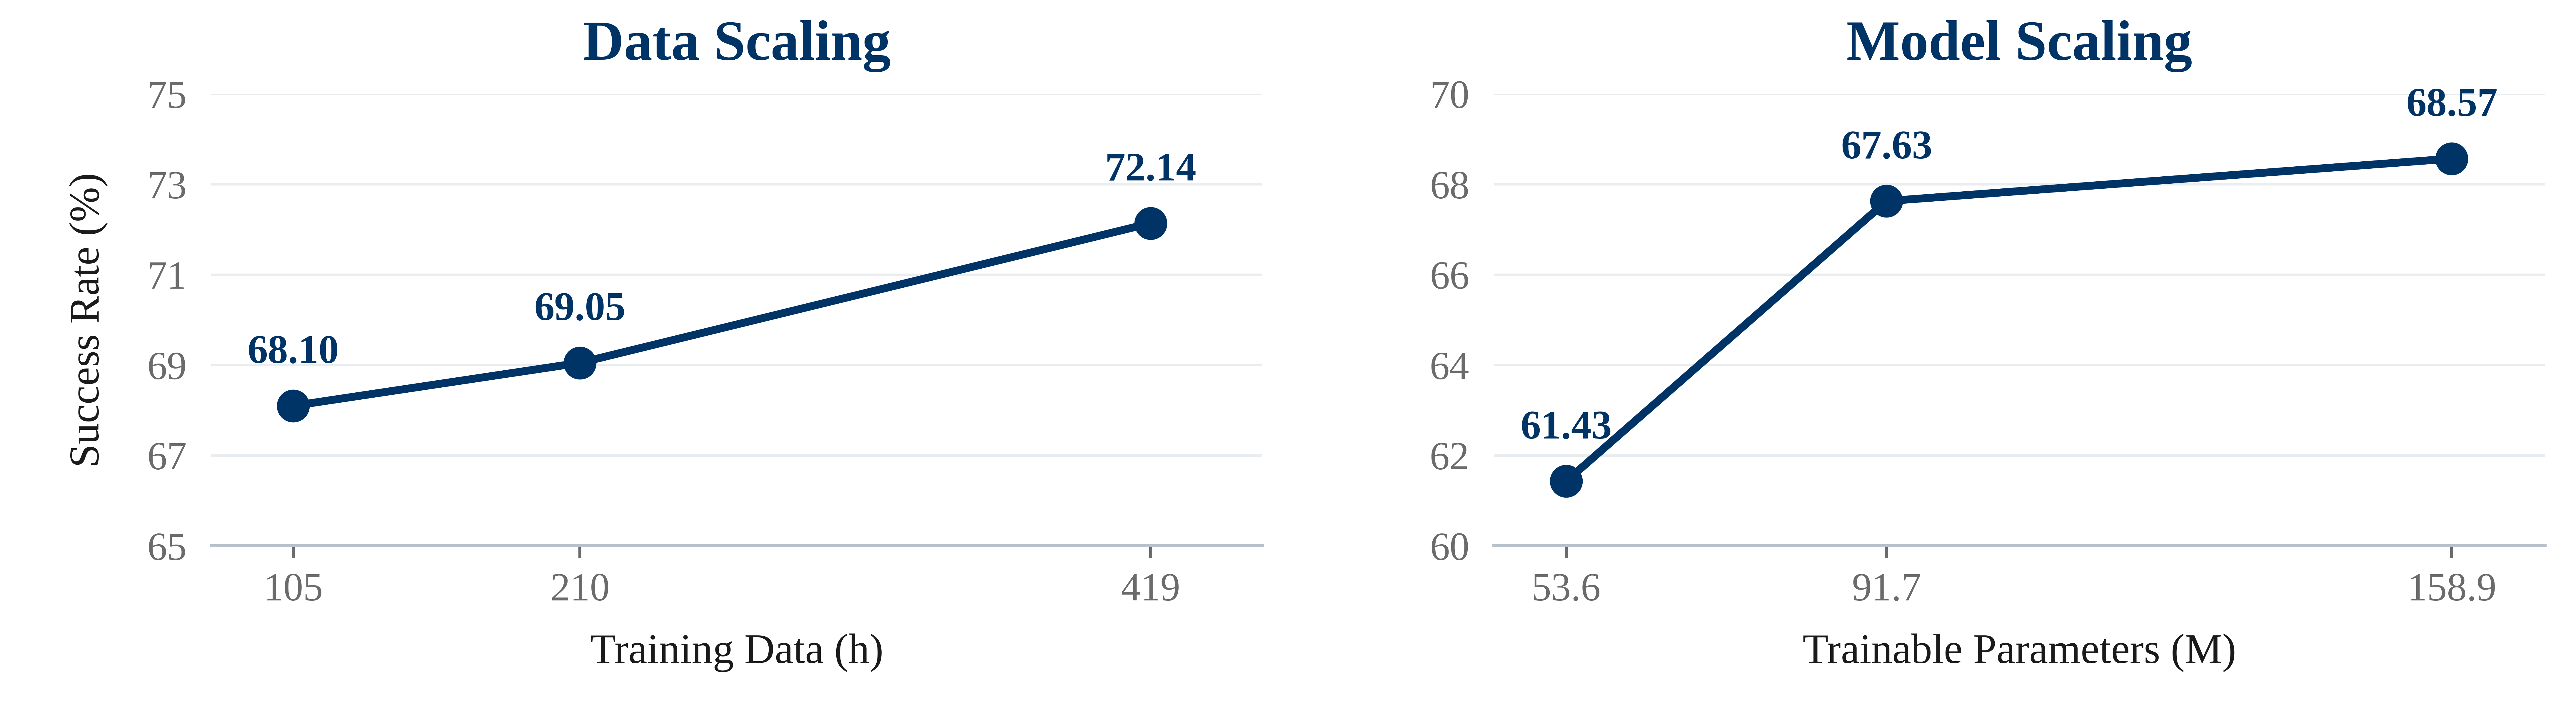
\includegraphics[width=\textwidth]{image/scaling_analysis.png}
\caption{\textbf{Separate scaling sweeps.} Left: policy-pretraining corpus duration. Right: active policy capacity (labeled trainable parameters in the source plot). Three tested scales show positive aggregate trends within each setting; no scaling-law fit is claimed.}
\label{fig:scaling}\end{figure*}

\subsection{Qualitative attention}
Figure~\ref{fig:attention} reproduces the source attention visualization. Kimodo-Policy's responses often lie near task-relevant regions, including balls, boxes, and interaction surfaces. These maps are qualitative illustrations. The source does not specify a common attribution calibration across architectures, so localization cannot establish causal reasoning or quantitative superiority over other policies.
\begin{figure*}[t]\centering
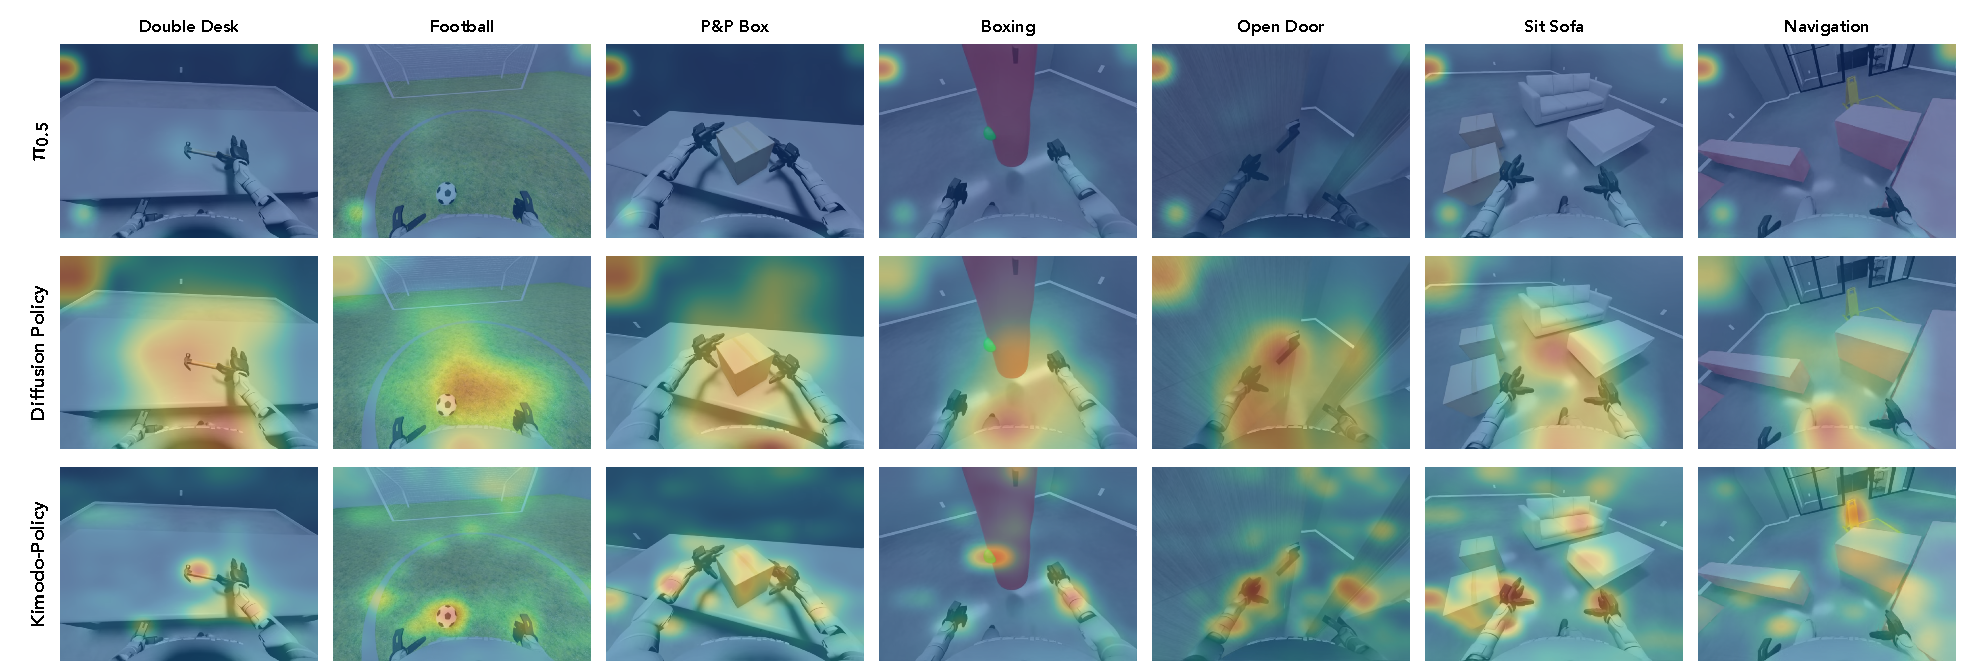
\includegraphics[width=\textwidth]{image/attention.pdf}
\caption{\textbf{Qualitative visual attention.} Columns show seven HumanoidArena tasks; rows compare $\pi_{0.5}$, DP, and Kimodo-Policy. Cross-model maps are illustrative rather than calibrated attribution measurements.}
\label{fig:attention}\end{figure*}

\subsection{Scope of the ablation evidence}
The main-paper ablation compares motion-prior removal, backbone unfreezing, the motion objective, root--body detachment, and extra policy pretraining on a three-task subset after joint training. It does not separately ablate the two visual-fusion paths, motion-history length, HandNet, or RTC. Lower reconstruction loss is not itself evidence of stronger closed-loop control. Generalization across low-level trackers and transfer from a human-skeleton generator without robot-space pretraining also remain unverified.
